\section{Appendix A: Supplementary Diagnostics Supporting the Core Claims}
\label{app:a}

This appendix is intentionally compact and retains only diagnostics that are most directly tied to the paper objective: translating temporal risk into auditable structural policy and subgroup diagnostics. It does not introduce new estimands, new policy regimes, or causal claims.

\subsection{Selection Rule for Supplementary Figures}

A figure is included in Appendix~A only if it satisfies at least one of the following conditions:
\begin{itemize}
\item it explains a key magnitude pattern reported in the main text;
\item it audits uncertainty for a reported structural contrast.
\end{itemize}

This rule keeps the appendix supportive rather than exploratory.

\subsection{A.1 Mechanism Diagnostics for the Policy Contrast}
\label{app:a_policy_mechanism}

The main text reports that the shock regime yields a substantially larger $\Delta S$ than the mechanism-aware regime under the default configuration. Figure~\ref{fig:app_policy_cov_deltas} is retained because it explains that difference mechanistically by showing the weekly covariate deltas induced by policy propagation.

\begin{figure}[!t]
\centering
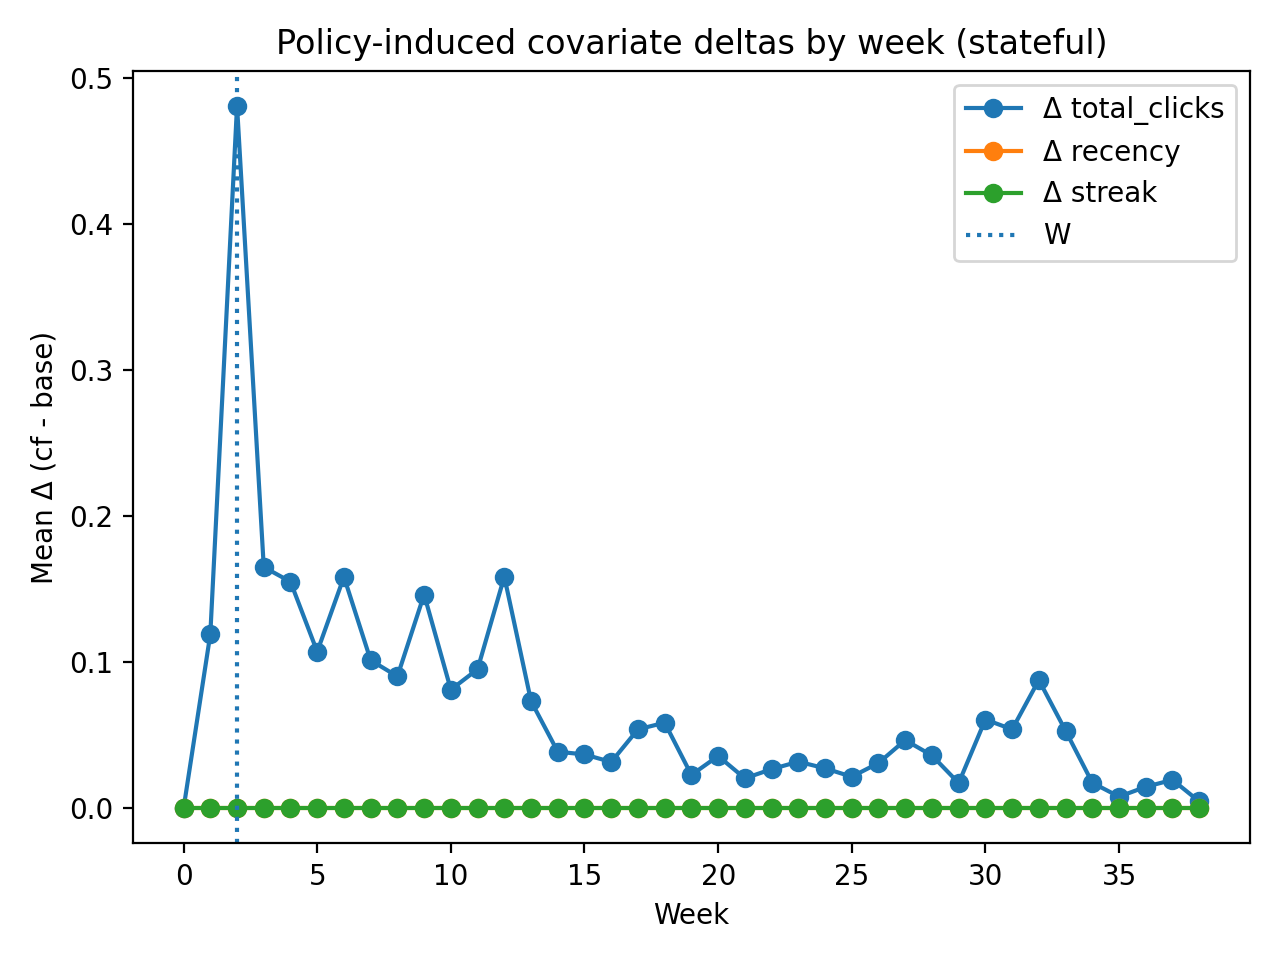
\includegraphics[width=0.45\textwidth]{outputs_v2/figures/fig_policy_covariate_deltas_by_week.png}
\caption{Supplementary mechanism diagnostics: weekly policy-induced covariate deltas. Small or short-lived deltas are consistent with weak mechanism-aware contrasts at $T_{policy}$ and negative mechanism-aware contrasts at $T_{eval\_policy}$ in the exported run.}
\label{fig:app_policy_cov_deltas}
\end{figure}

The associated numeric summaries are reported in the
\texttt{outputs\_v2/tables} artifact folder, specifically in
\texttt{table\_policy\_covariate\_deltas\_by\_week.csv}
and
\texttt{table\_policy\_activation\_summary.csv}.
This block is included because it strengthens interpretability: it shows how the simulated intervention propagates through the state variables and why the resulting structural contrast remains small in the mechanism-aware case.

\subsection{A.2 Bootstrap Uncertainty Audit for RQ3}
\label{app:a_rq3_bootstrap}

Figure~\ref{fig:app_boot_tp} is retained because it audits the stability of the subgroup change-in-gap signal reported for RQ3 at the primary horizon.

\begin{figure}[!t]
\centering
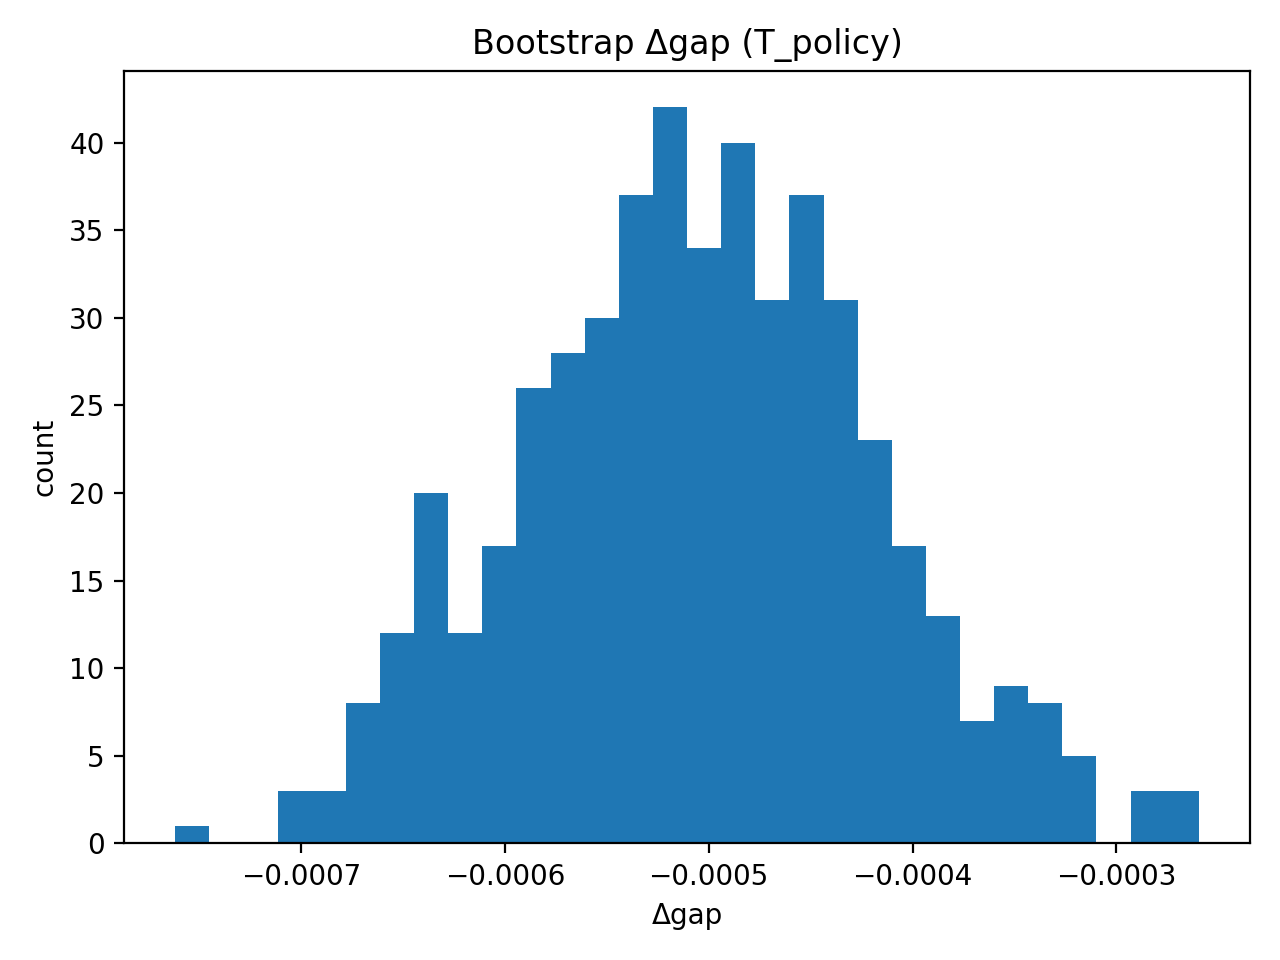
\includegraphics[width=0.45\textwidth]{outputs_v2/figures/fig_rq3_bootstrap_hist_deltagap_Tpolicy.png}
\caption{Bootstrap distribution of $\Delta Gap(T_{policy})$. Included to audit uncertainty for the subgroup contrast at the primary reporting horizon.}
\label{fig:app_boot_tp}
\end{figure}

The compact confidence-interval summaries are reported in
\texttt{rq3\_policy\_bootstrap\_wide.csv}, available in the
\texttt{outputs\_v2/tables} artifact folder, including both $T_{policy}$ and $T_{eval\_metrics}$ summaries. This block does not introduce a new subgroup result; it makes uncertainty auditing explicit.

\subsection{A.3 Appendix Boundary}

Appendix~A is intentionally constrained to diagnostics with the highest relevance to the core argument. Additional diagnostics (for example, IPCW calibration robustness and calibration-by-group) remain available in the exported artifact package under \texttt{outputs\_v2/figures} and \texttt{outputs\_v2/tables}, but are omitted here to keep the appendix focused.

Accordingly, all conclusions remain within the same contract used throughout the paper: the reported quantities are \textit{model-implied simulated regime contrasts} under explicit protocol rules, and the appendix serves only to strengthen the evidentiary basis for reading those contrasts.